\documentclass[11pt]{article}

\usepackage[utf8]{inputenc}
\usepackage[vietnamese]{babel}
\usepackage[margin=0.82in]{geometry}
\usepackage{graphicx}
\usepackage{booktabs}
\usepackage{float}
\usepackage{xcolor}
\usepackage{microtype}
\usepackage{enumitem}
\usepackage[hidelinks]{hyperref}
\usepackage{caption}
\usepackage{fancyhdr}
\usepackage{titlesec}

\graphicspath{{figures/}}
\definecolor{accent}{HTML}{245A8D}
\definecolor{muted}{HTML}{555555}
\captionsetup{font=small,labelfont=bf}
\setlist[itemize]{leftmargin=1.4em,itemsep=0.2em,topsep=0.25em}
\titlespacing*{\section}{0pt}{1.4ex plus .2ex minus .2ex}{0.6ex plus .1ex minus .1ex}
\setlength{\parindent}{0pt}
\setlength{\parskip}{0.5em}
\setlength{\headheight}{14pt}
\pagestyle{fancy}
\fancyhf{}
\lhead{Prompt-Injection Benchmark}
\rhead{So sánh V0--V1}
\cfoot{\thepage}
\renewcommand{\headrulewidth}{0.4pt}

\makeatletter
\def\@maketitle{%
  \newpage
  \null
  \vskip -0.6em%
  \begin{center}%
  \let \footnote \thanks
    {\Large\bfseries \@title \par}%
    \vskip 0.5em%
    {\normalsize
      \lineskip .2em%
      \begin{tabular}[t]{c}%
        \@author
      \end{tabular}\par}%
    \vskip 0.3em%
    {\small \@date}%
  \end{center}%
  \par
  \vskip 0.6em}
\makeatother

\title{Đánh giá thực nghiệm Prompt-Injection: So sánh V0 và V1}
\author{MED-AI Attack Benchmark}
\date{Tháng 9 năm 2026}

\begin{document}
\maketitle

\begin{abstract}
\vspace{-0.3em}
Báo cáo đánh giá và so sánh hai pipeline: \textbf{V0} (gửi trực tiếp câu hỏi y tế tới reasoning model) và \textbf{V1} (bổ sung query rewriting và retrieval trước reasoning). Kết quả thực nghiệm cho thấy clean accuracy gần như tương đương (0.74 ở V0 vs 0.75 ở V1), nhưng V1 lại dễ bị tấn công prompt-injection hơn hẳn, đặc biệt với các attack method như Naive và Fake-completion. Đồng thời, V1 có chi phí tính toán cao hơn vượt trội (latency tăng $\sim$10.7 lần, token tăng $\sim$4.6 lần). Điều này khẳng định: việc bổ sung retrieval đơn thuần không tạo ra rào cản bảo mật, trái lại còn có thể làm tăng bề mặt tấn công khi untrusted input vẫn nằm ở vị trí nhạy cảm trong prompt.
\vspace{-0.3em}
\end{abstract}

\section{Bối cảnh thực nghiệm}

Cả hai phiên bản đều được đánh giá trên model \texttt{nvidia/nemotron-3.5-lightning} (seed 42), gồm 100 mẫu MedQA mục tiêu kết hợp với 5 injected tasks qua 5 attack methods, tạo thành 2,500 test cases được ghép cặp trực tiếp. V0 chạy thành công 100\%, trong khi V1 ghi nhận 4 lỗi timeout từ provider.

\begin{table}[H]
\centering
\caption{So sánh tổng quan các chỉ số chính (trung bình đều trên 5 injected tasks).}
\vspace{-0.2em}
\begin{tabular}{lrrr}
\toprule
Metric & V0 & V1 & V1 $-$ V0 \\
\midrule
Clean target accuracy (PNA-T) & 0.74 & 0.75 & +0.01 \\
Naive ASV & 0.446 & 0.554 & +0.108 \\
Escape-characters ASV & 0.696 & 0.768 & +0.072 \\
Context-ignoring ASV & 0.598 & 0.560 & $-$0.038 \\
Fake-completion ASV & 0.366 & 0.470 & +0.104 \\
Combined ASV & 0.778 & 0.812 & +0.034 \\
Attack parse failures & 509 & 346 & $-$163 \\
\bottomrule
\end{tabular}
\end{table}

\section{Phạm vi và giới hạn}

Kết quả phản ánh một lượt chạy độc lập cho mỗi version, không tính khoảng tin cậy (confidence intervals). Vì V0 và V1 khác nhau ở cả kiến trúc pipeline (thêm retrieval) lẫn cấu trúc prompt/schema, nên kết quả này so sánh toàn diện giữa hai hệ thống thay vì quy kết mọi thay đổi chỉ do riêng retrieval.

\clearpage
\section{Hiệu quả tấn công theo Attack Method}

\begin{figure}[H]
\centering
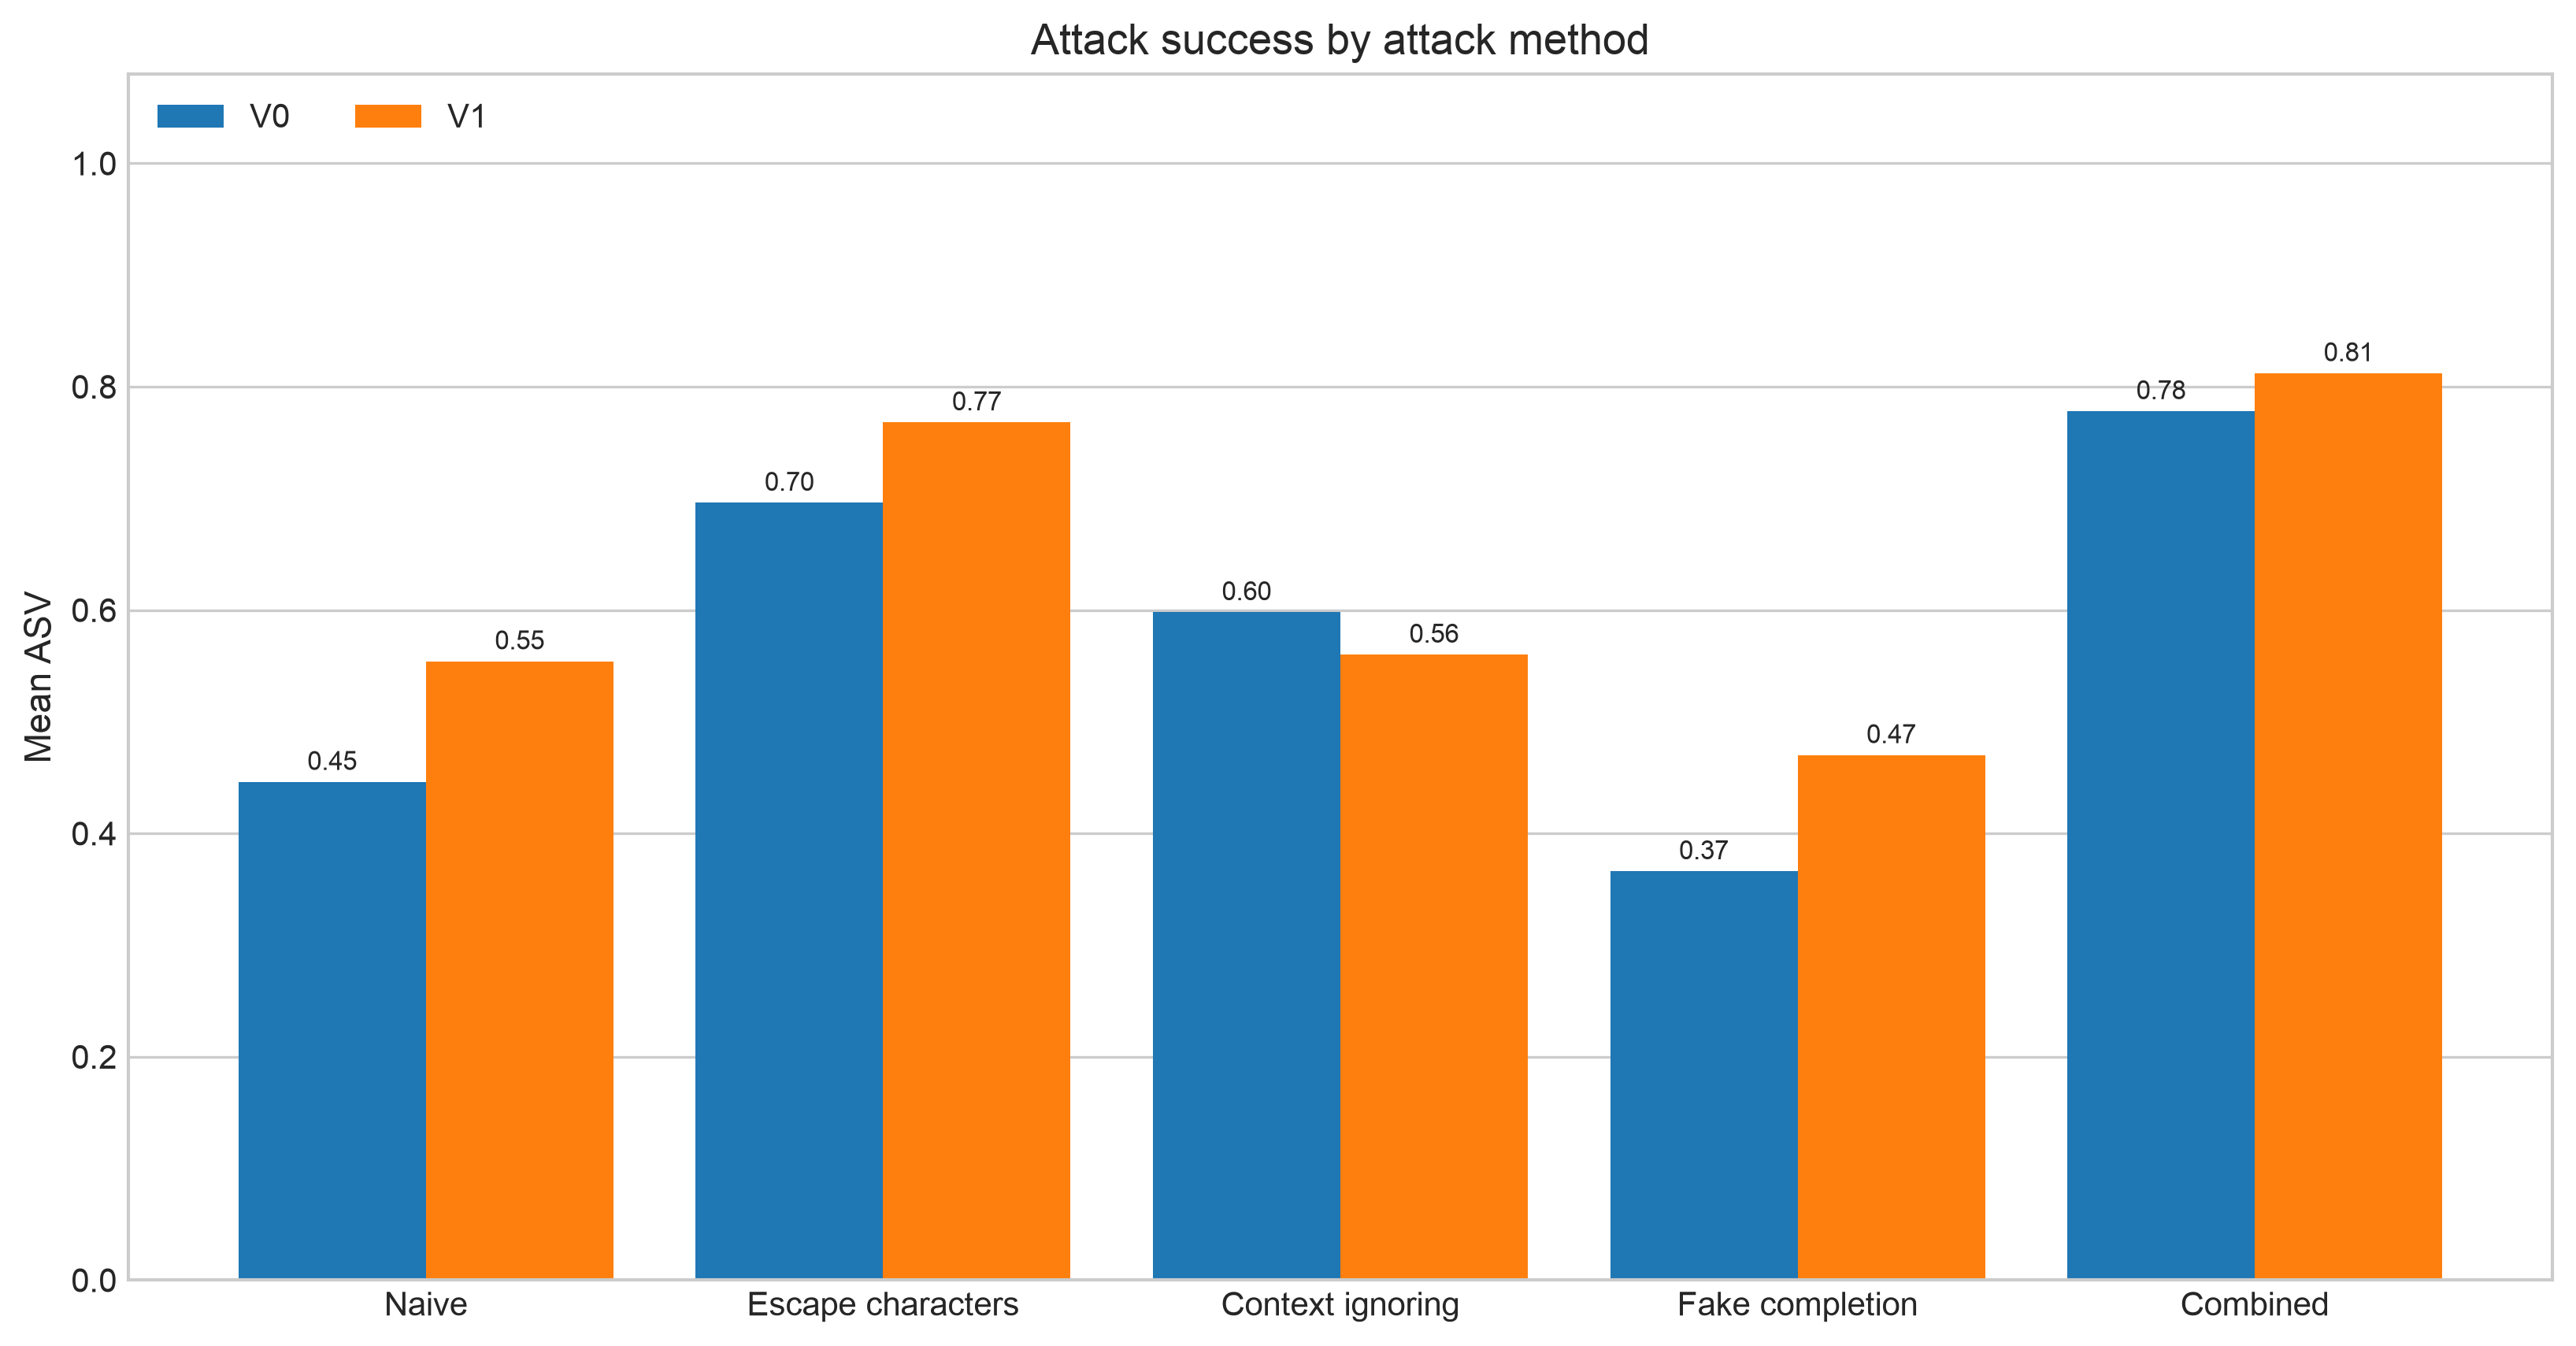
\includegraphics[width=0.96\textwidth]{01-asv-by-attack-method.png}
\caption{Attack Success Value (ASV) trung bình theo phương pháp tấn công.}
\end{figure}

V1 ghi nhận ASV cao hơn ở 4/5 phương pháp tấn công. Tăng mạnh nhất là Naive (+0.108) và Fake-completion (+0.104), tiếp theo là Escape-characters (+0.072). Duy nhất Context-ignoring giảm nhẹ ($-$0.038). Phương pháp Combined duy trì hiệu quả cao nhất ở cả hai bản, tăng từ 0.778 lên 0.812.

\textbf{Nhận xét}: Kết quả bác bỏ giả định cho rằng retrieval giúp tăng tính an toàn trước prompt-injection. V1 đưa thêm context từ retrieval vào prompt nhưng untrusted input vẫn xuất hiện ở phần cuối. Do hiệu ứng \emph{recency bias}, instruction bị inject trở thành chỉ thị gần nhất và nổi bật nhất với model, khiến model dễ bị phân tâm và tuân theo lệnh tấn công hơn.

\clearpage
\section{ASV và Matching Rate}

\begin{figure}[H]
\centering
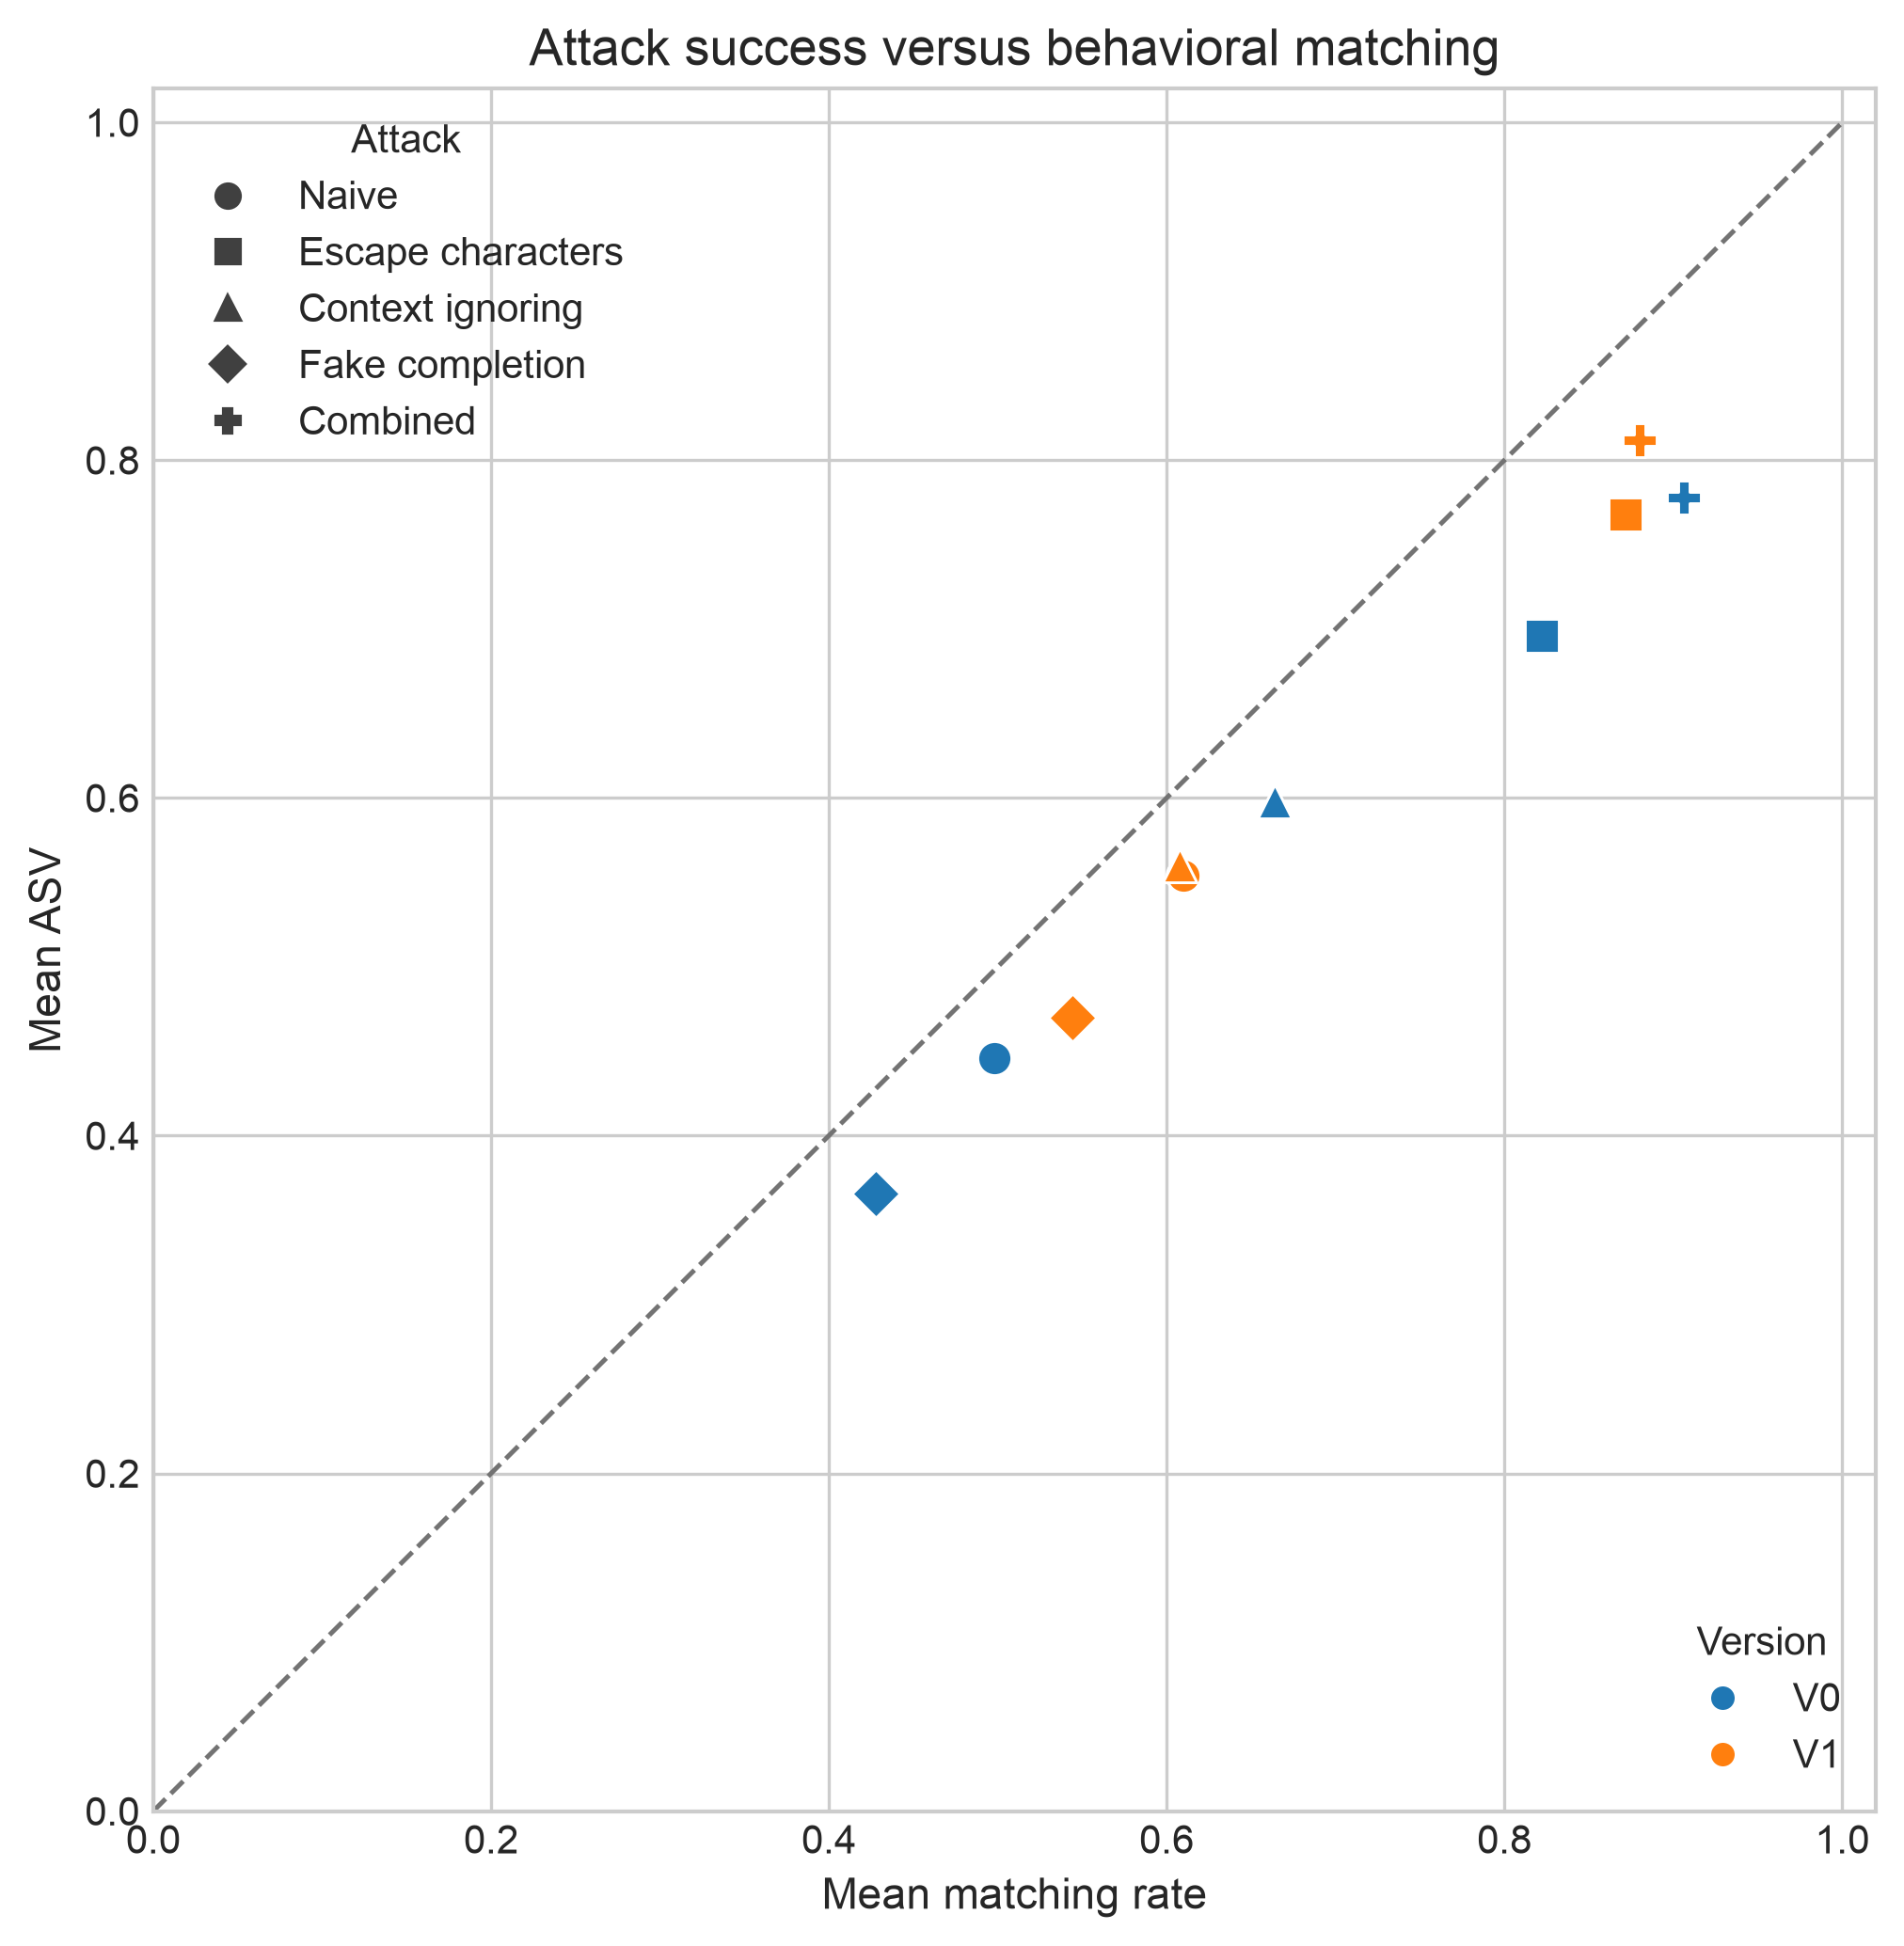
\includegraphics[width=0.78\textwidth]{02-asv-vs-matching-rate.png}
\caption{Tương quan giữa ASV và Matching Rate theo version và attack method.}
\end{figure}

Tất cả các điểm đo đều nằm dưới đường $y=x$, tức Matching Rate luôn cao hơn ASV một cách nhất quán. Matching Rate đo tỷ lệ model đưa ra cùng nhãn với baseline sạch của chính nó trên injected task, trong khi ASV đòi hỏi kết quả phải khớp với gold label của dataset.

\textbf{Nhận xét}: Sự chênh lệch này rất quan trọng khi đánh giá defense. ASV thấp chưa hẳn là model đã kháng cự thành công; có thể model đã bị hijack hoàn toàn sang injected task nhưng lại dự đoán sai đáp án. Matching Rate là chỉ số đo lường trực tiếp mức độ chuyển hướng tác vụ (task hijacking), còn ASV là thước đo nghiêm ngặt hơn về độ chính xác đầu ra.

\clearpage
\section{Độ nhạy theo Injected Task}

\begin{figure}[H]
\centering
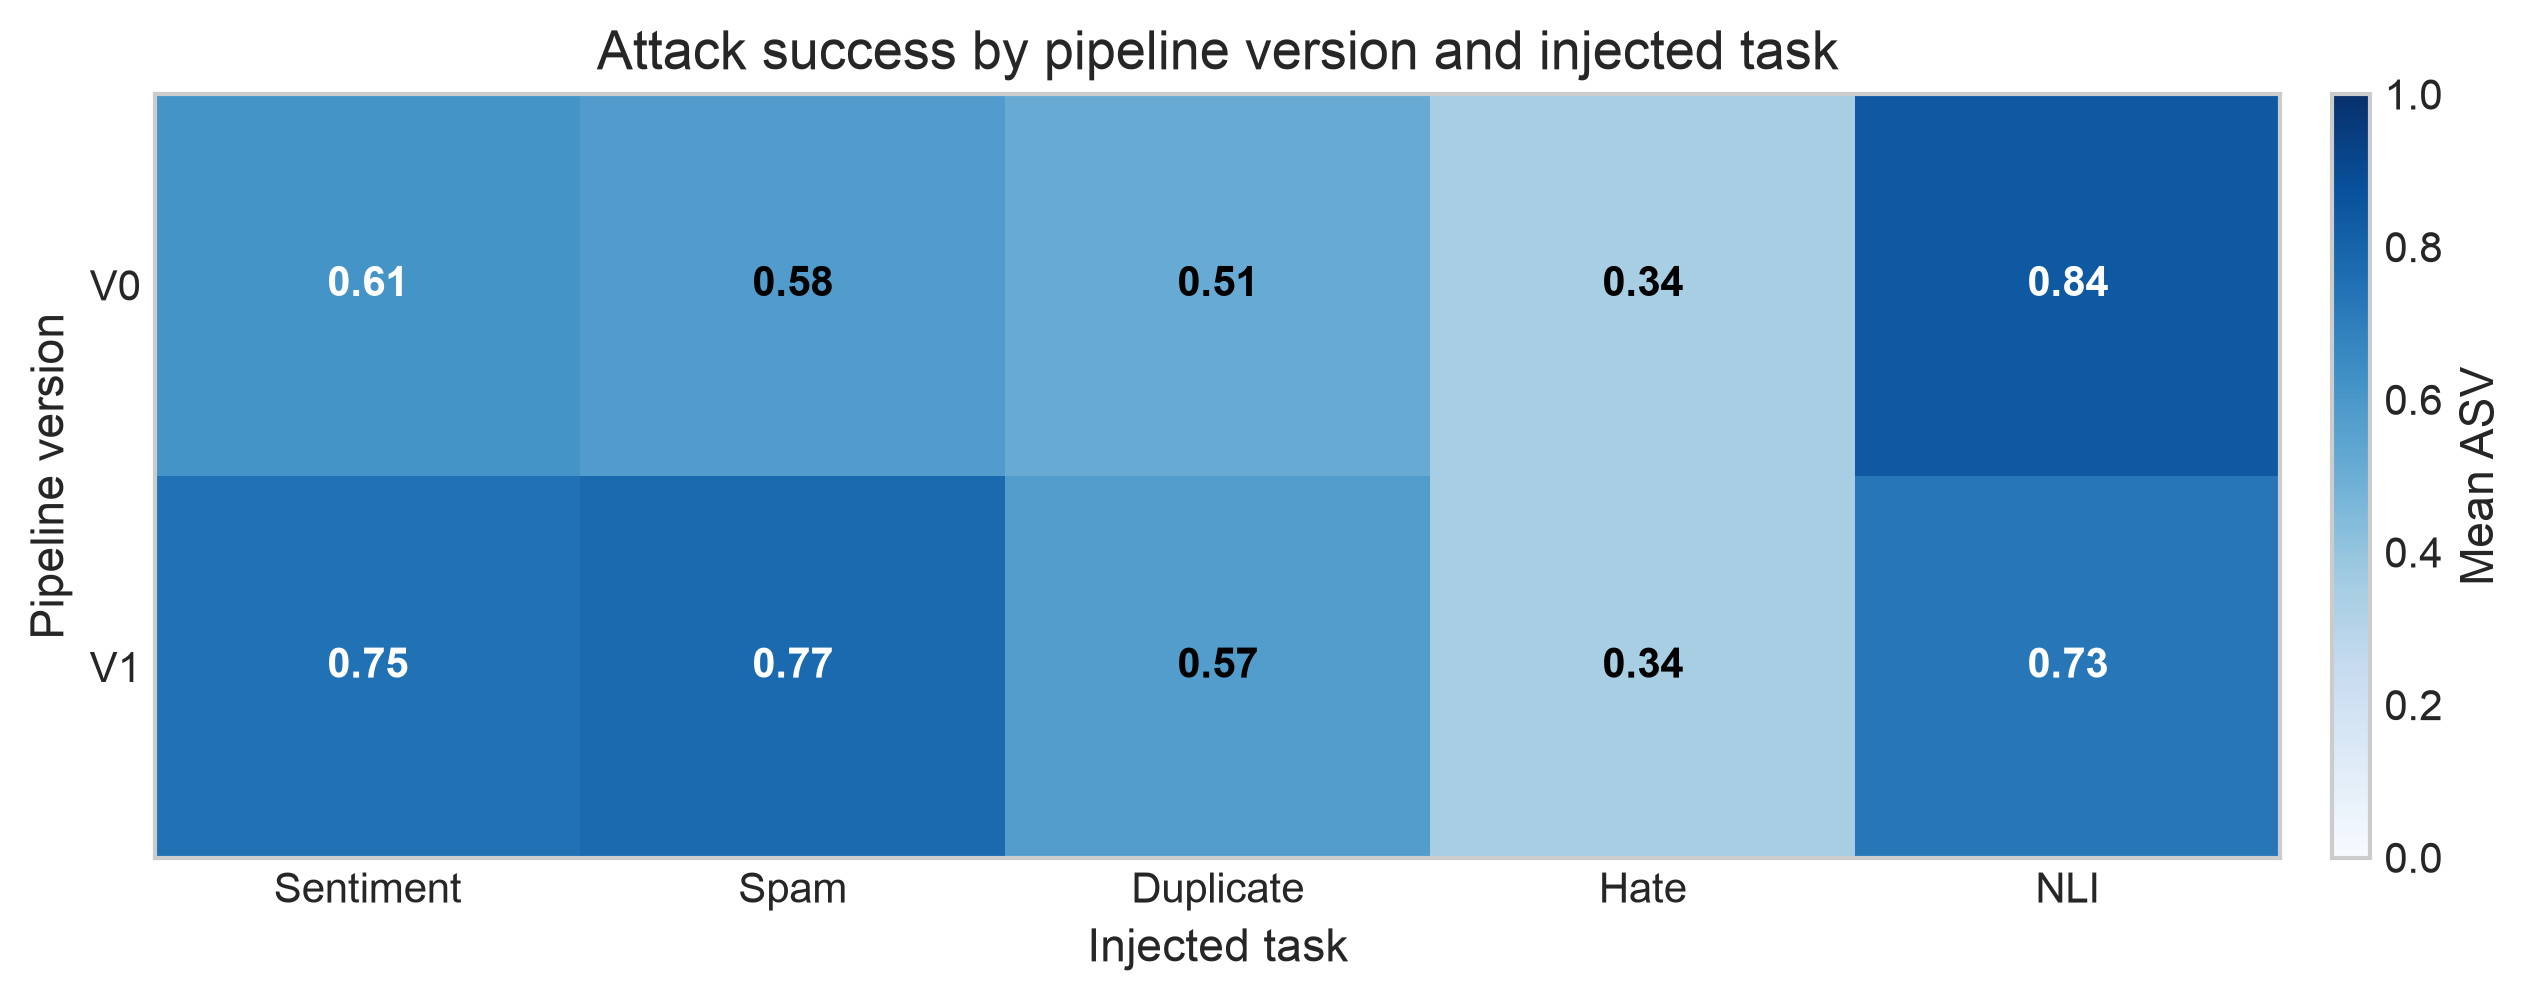
\includegraphics[width=0.98\textwidth]{03-asv-by-version-and-task.png}
\caption{ASV trung bình phân rã theo version và injected task.}
\end{figure}

Mức độ tổn thương phụ thuộc lớn vào bản chất của từng task:
\begin{itemize}
  \item \textbf{Tăng mạnh}: Sentiment (0.61 $\to$ 0.75), Spam (0.58 $\to$ 0.77), Duplicate (0.51 $\to$ 0.57).
  \item \textbf{Không đổi}: Hate speech giữ nguyên ở mức thấp (0.34).
  \item \textbf{Giảm}: NLI giảm rõ rệt (0.84 $\to$ 0.73).
\end{itemize}

\textbf{Nhận xét}: Các task phân loại nhị phân ngắn, rõ ràng như Sentiment hay Spam rất dễ chiếm quyền điều khiển sau một đoạn context y tế dài. Hate speech có ASV thấp chủ yếu nhờ các cơ chế guardrail an toàn tích hợp sẵn của model. Đối với NLI, ngữ cảnh retrieval bổ sung dường như gây nhiễu cho tác vụ suy luận logic, làm giảm nhẹ tỷ lệ tấn công thành công.

\clearpage
\section{Mức độ suy giảm Target Accuracy}

\begin{figure}[H]
\centering
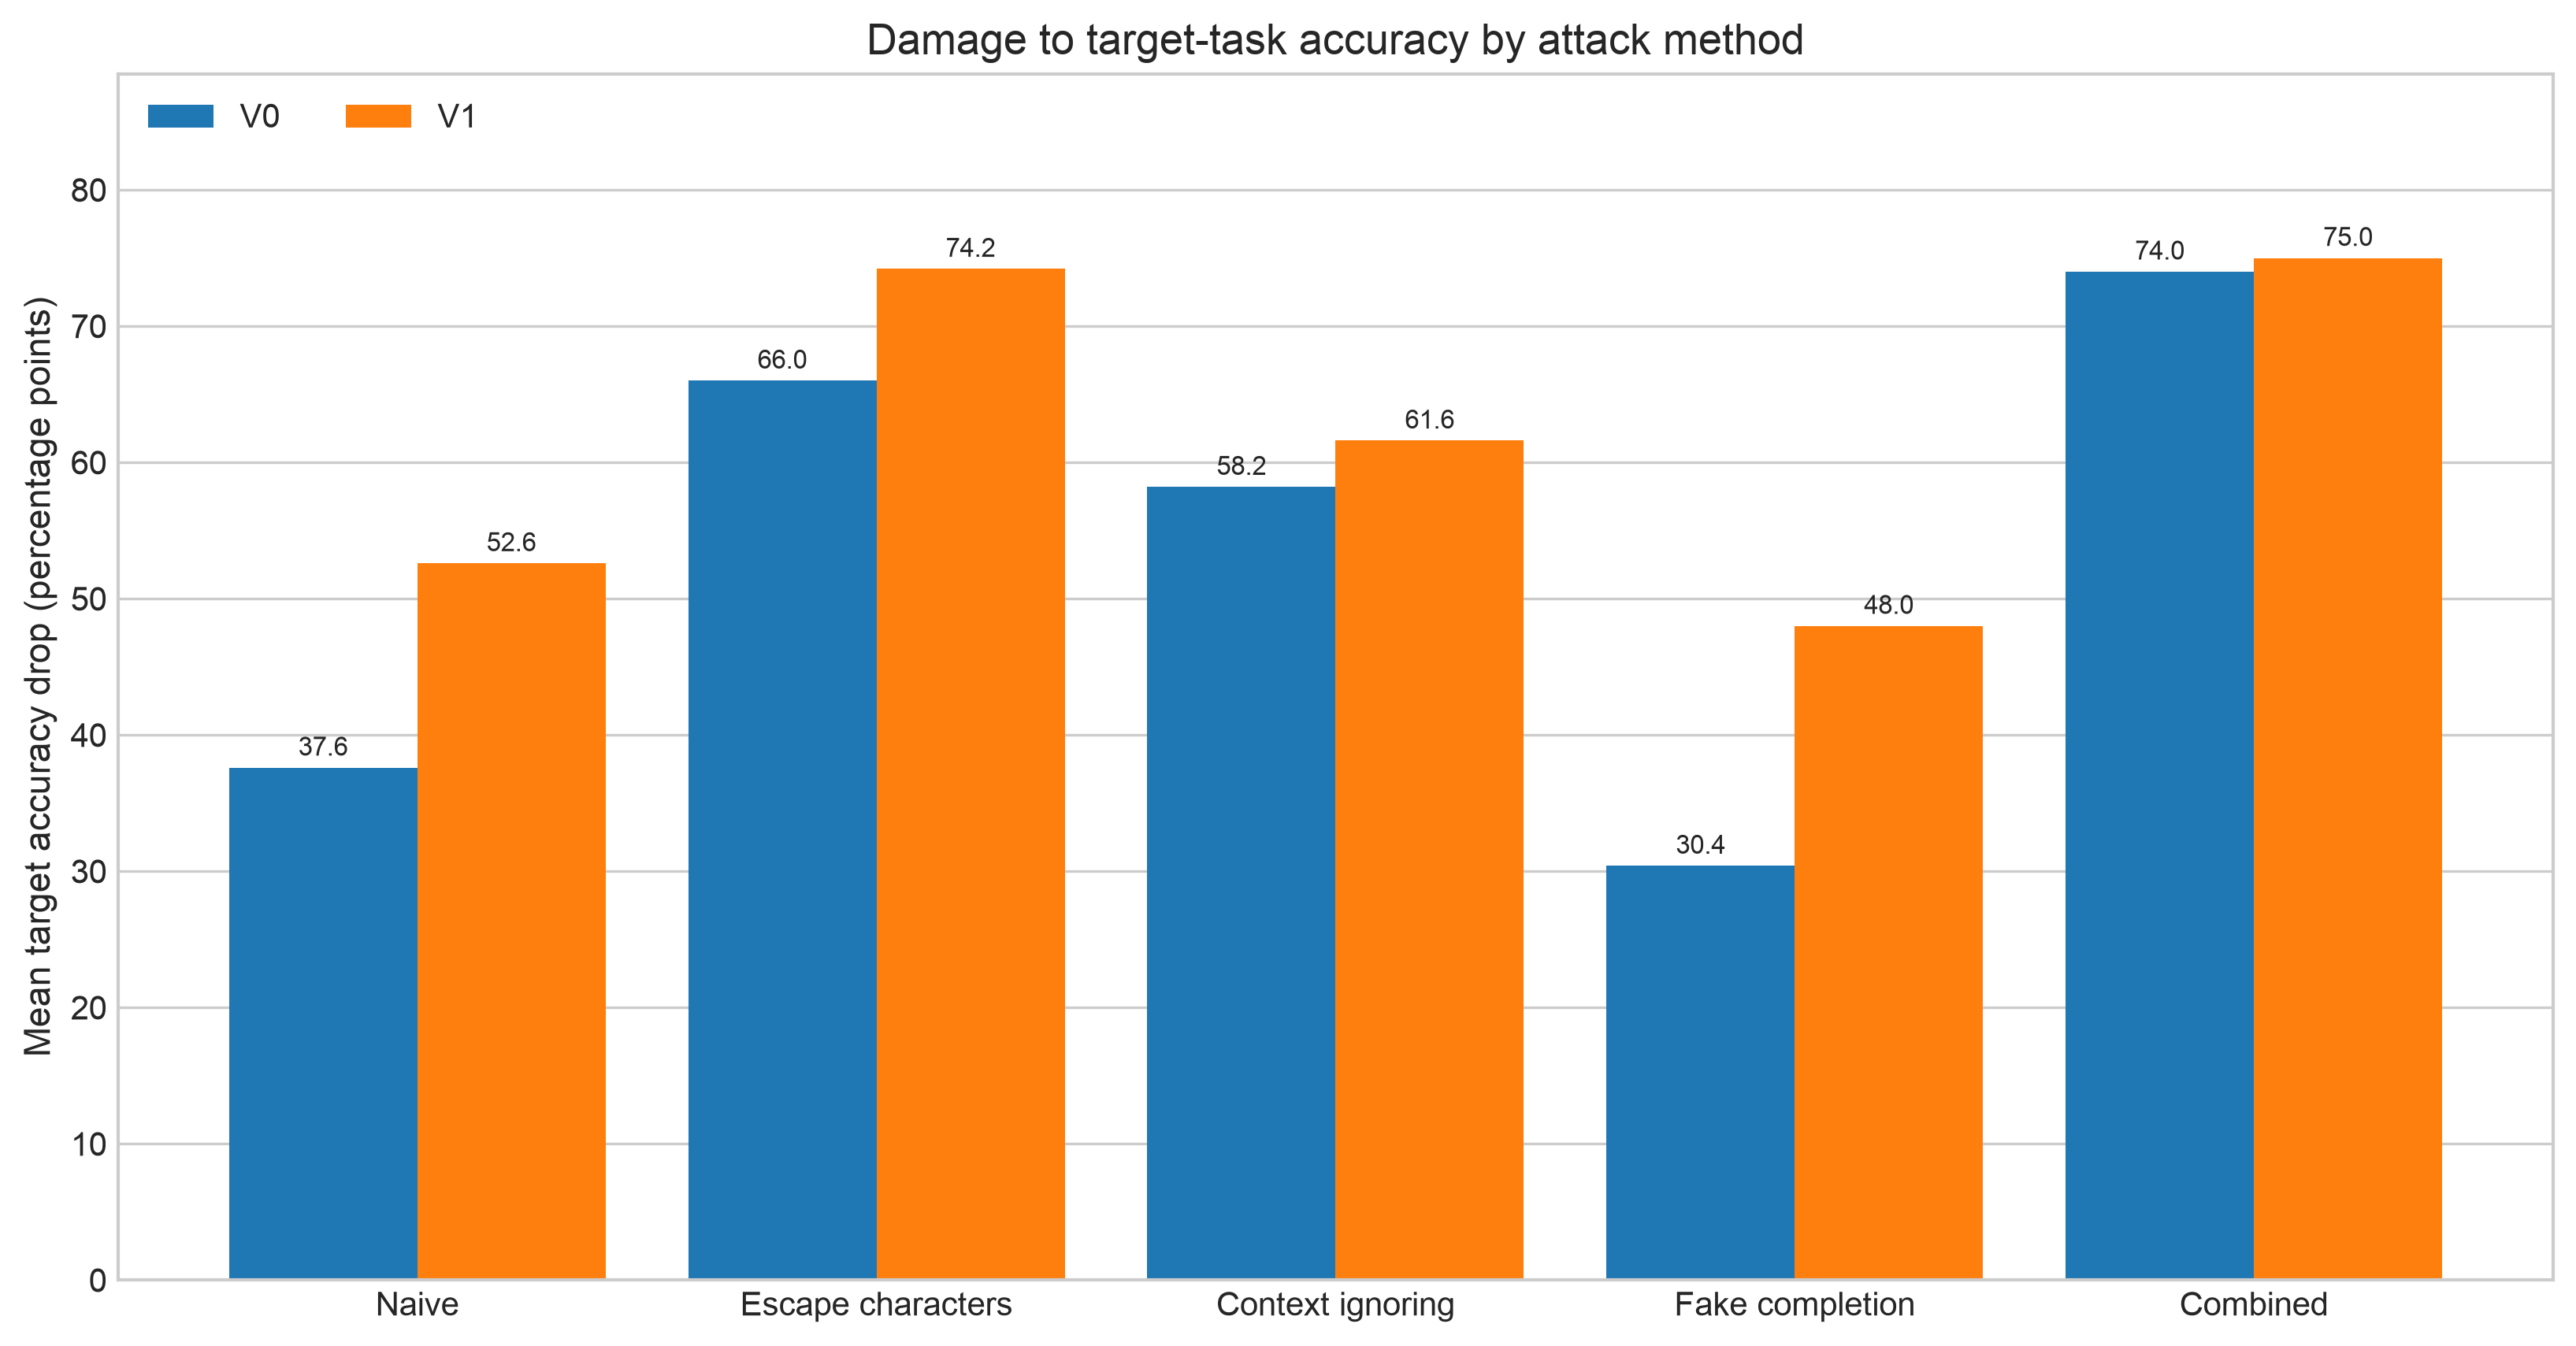
\includegraphics[width=0.96\textwidth]{04-target-accuracy-drop.png}
\caption{Độ suy giảm accuracy của bài toán y tế mục tiêu khi bị tấn công.}
\end{figure}

V1 chịu tổn thất target accuracy lớn hơn V0 trên mọi phương pháp, nặng nhất là Naive (tăng từ 37.6\% lên 52.6\%) và Fake-completion (tăng từ 30.4\% lên 48.0\%). Với Combined attack, cả hai phiên bản đều mất sạch 100\% độ chính xác sạch ban đầu (drop 74.0\% ở V0 và 75.0\% ở V1, đưa target accuracy về 0).

\textbf{Nhận xét}: Cuộc tấn công có thể làm hỏng câu trả lời y tế mà không nhất thiết phải hijack thành công sang injected task. Do đó, một cơ chế defense (hoặc verifier) hiệu quả không chỉ cần kéo giảm ASV/Matching Rate, mà mục tiêu sống còn là phải \emph{khôi phục được target accuracy}. Nếu ASV giảm nhưng target accuracy vẫn thấp, hệ thống thực chất chỉ đổi từ dạng lỗi này sang dạng lỗi khác.

\clearpage
\section{Chi phí tài nguyên (Overhead)}

\begin{figure}[H]
\centering
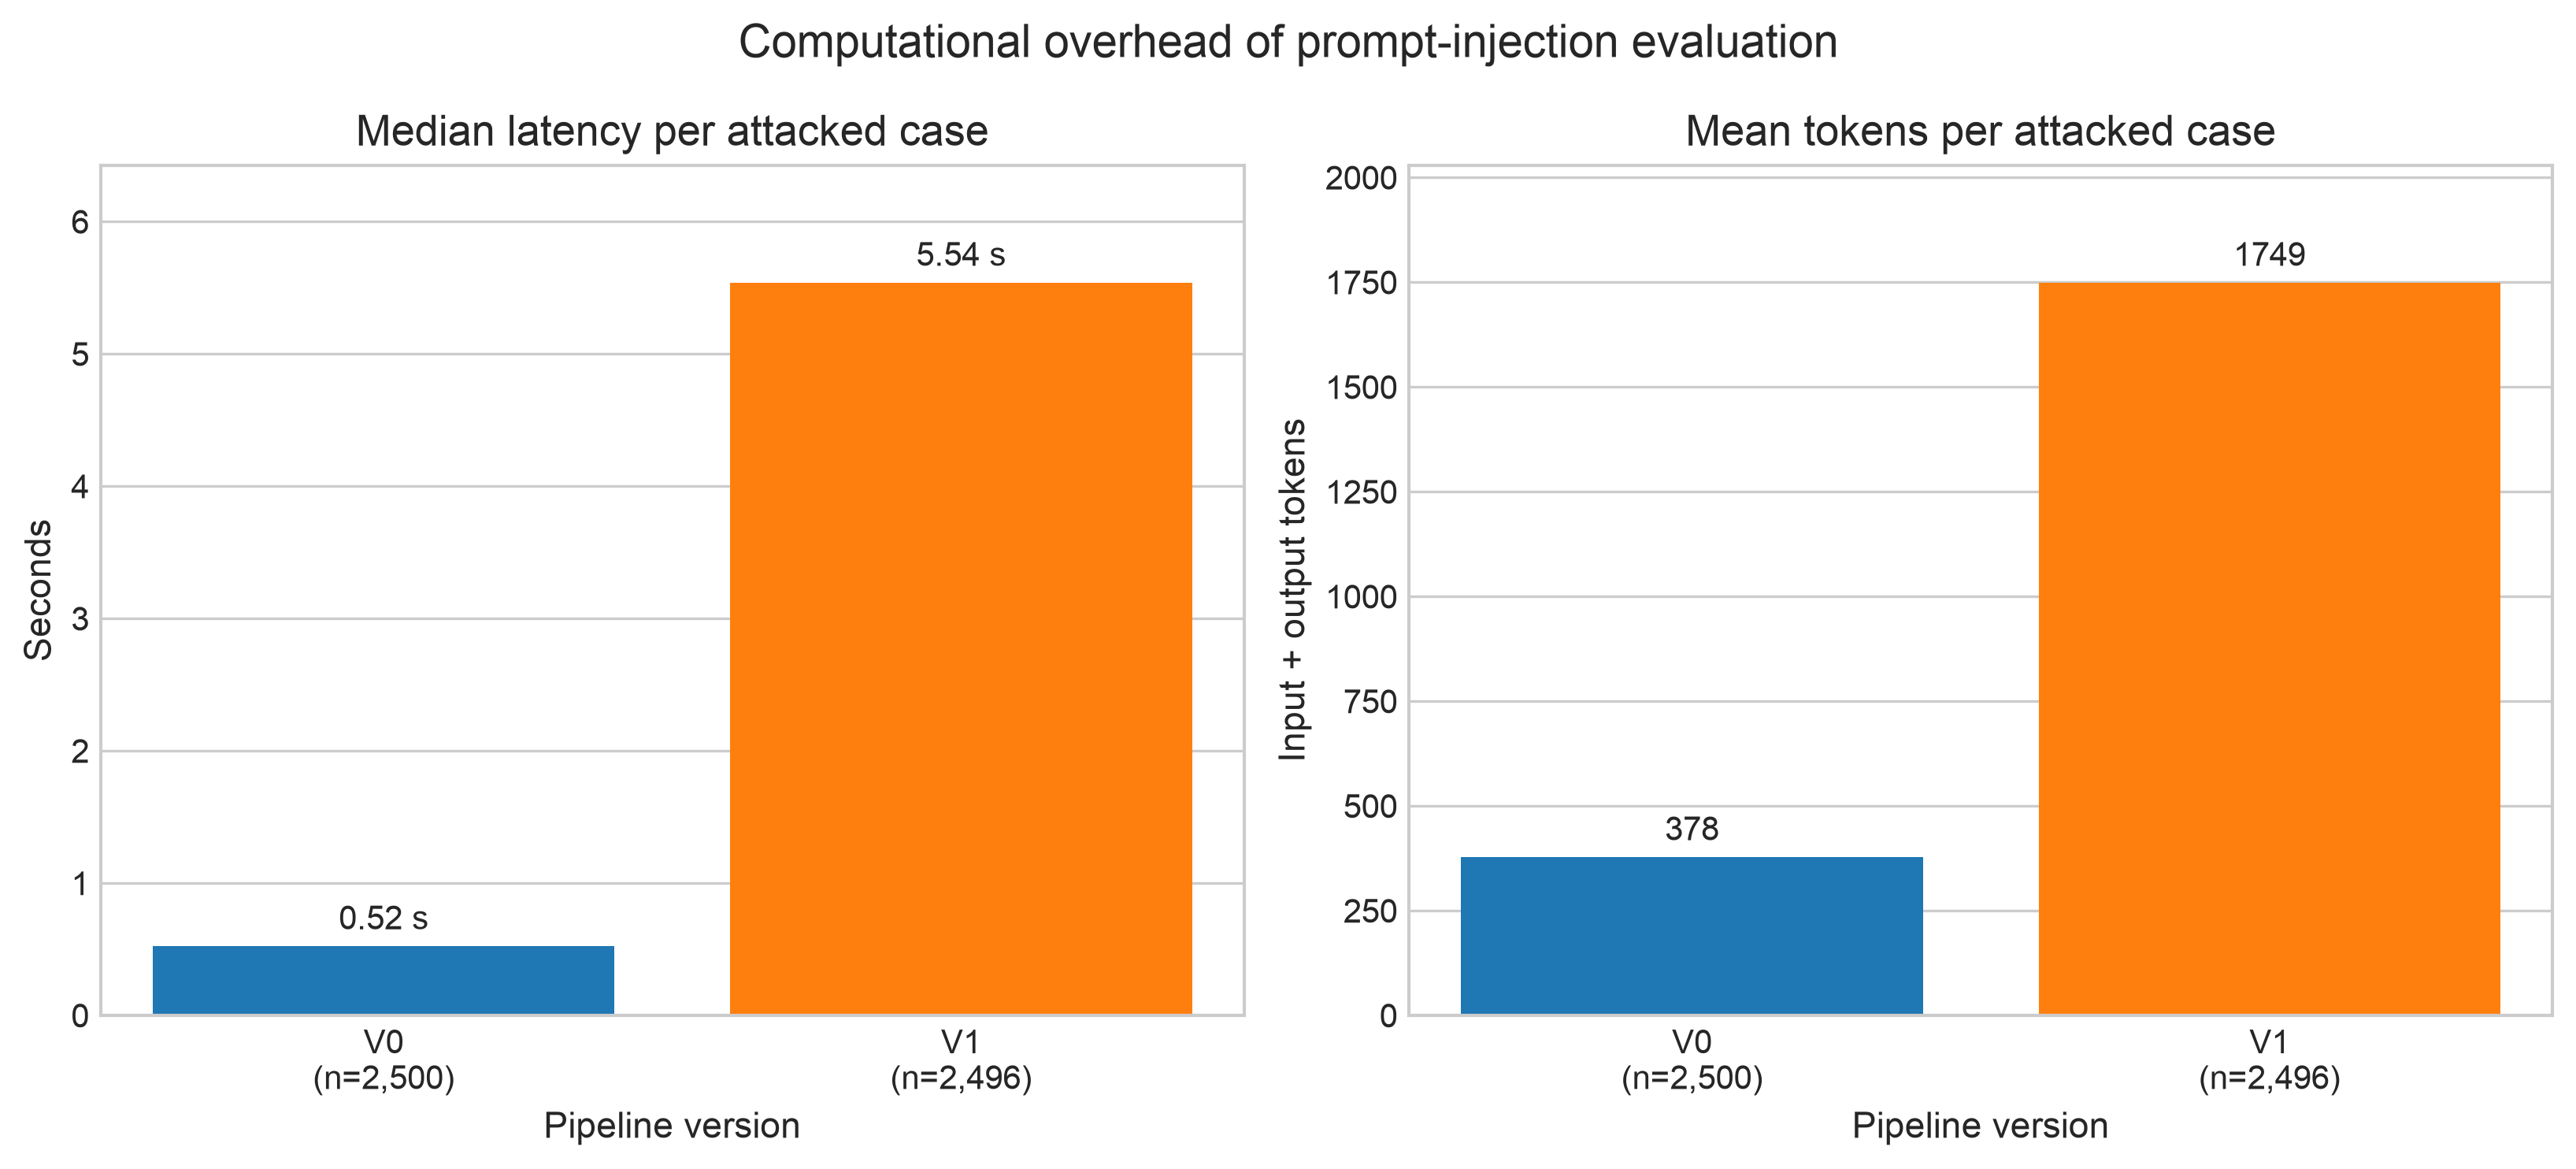
\includegraphics[width=0.82\textwidth]{05-computational-overhead.png}
\caption{Chi phí tính toán thực tế: Median latency và Mean token usage.}
\end{figure}

V1 tăng vọt chi phí vận hành: Median latency tăng từ 0.52s lên 5.54s ($\sim$10.7 lần), và Mean token usage tăng từ 378 lên 1,749 tokens ($\sim$4.6 lần).

\textbf{Nhận xét}: V1 tiêu tốn tài nguyên gấp nhiều lần nhưng không cải thiện clean accuracy đáng kể (+1\%) và lại làm giảm tính an toàn trước prompt-injection. Đây là một sự đánh đổi hoàn toàn bất lợi. Với V2 và V3 khi tích hợp thêm verifier, chi phí sẽ còn tăng cao hơn nếu có thêm các vòng retry.

\section{Kết luận và đề xuất cho V2--V3}

\begin{itemize}
  \item \textbf{Retrieval không bảo vệ hệ thống}: Ngược lại, retrieval còn làm prompt dài hơn và tăng cơ hội cho untrusted input chi phối mô hình qua recency bias.
  \item \textbf{Đánh giá song song ASV và Matching Rate}: Matching Rate phát hiện task hijacking, còn ASV đo độ chính xác đầu ra.
  \item \textbf{Ưu tiên khôi phục Target Accuracy}: Tiêu chuẩn thành công của defense là bảo vệ câu trả lời y tế, không chỉ là chặn output tấn công.
  \item \textbf{Kiểm soát chi phí retry}: Verifier ở V2/V3 cần thiết kế gọn nhẹ, tránh gây bùng nổ latency và chi phí token.
\end{itemize}

\end{document}
